\documentclass[sigconf]{acmart}

\settopmatter{printacmref=false} % Removes citation information below abstract
\renewcommand\footnotetextcopyrightpermission[1]{} % removes footnote with conference information in first column
\pagestyle{plain} % removes running headers

\usepackage{booktabs} % For formal tables

\usepackage{subcaption} % for multiple subfigures
\usepackage{footnote}
\makesavenoteenv{tabular}
\makesavenoteenv{table}


% Copyright
\setcopyright{none}
%\setcopyright{acmcopyright}
%\setcopyright{acmlicensed}
%\setcopyright{rightsretained}
%\setcopyright{usgov}
%\setcopyright{usgovmixed}
%\setcopyright{cagov}
%\setcopyright{cagovmixed}


% DOI
%\acmDOI{10.475/123_4}

% ISBN
%\acmISBN{123-4567-24-567/08/06}

%Conference
%\acmConference[Short Name N/A]{Long Name N/A}{Date N/A}{Location N/A}
%\acmYear{N/A}
%\copyrightyear{2018}


%\acmArticle{N/A}
%\acmPrice{N/A}

% These commands are optional
%\acmBooktitle{Transactions of the ACM Woodstock conference}
%\editor{Jennifer B. Sartor}
%\editor{Theo D'Hondt}
%\editor{Wolfgang De Meuter}


\begin{document}
\title{A Covert Channel Detector for Machine Learning Models}
%\titlenote{Produces the permission block, and
  %copyright information}
%\subtitle{Extended Abstract}
%\subtitlenote{The full version of the author's guide is available as
  %\texttt{acmart.pdf} document}


\author{John Stein}
%\authornote{Dr.~Trovato insisted his name be first.}
%\orcid{1234-5678-9012}
\affiliation{%
  \institution{Indiana University}
  \streetaddress{107 S Indiana Ave}
  \city{Bloomington}
  \state{Indiana}
  \postcode{47405}
}
\email{jodstein@iu.edu}

%\author{David Crandall, PhD}
%%\authornote{The secretary disavows any knowledge of this author's actions.}
%\affiliation{%
%  \institution{Indiana University}
%  \streetaddress{107 S Indiana Ave}
%  \city{Bloomington}
%  \state{Indiana}
%  \postcode{47405}
%}
%\email{djcran@indiana.edu}

% The default list of authors is too long for headers.
%\renewcommand{\shortauthors}{B. Trovato et al.}


\begin{abstract}
It has been shown that malicious model training code can augment sensitive training data with specially-crafted samples to enable later exfiltration of the sensitive data by an attacker who has black-box access to the completed model, but no direct access to the sensitive training data. \cite{DBLP:journals/corr/abs-1709-07886}  This is known as a Covert Channel for machine learning models.  It has also been shown an attacker can infer whether a specific sample was included in the training set for a black-box model if the attacker has knowledge of the model's structure or can generate models with similar structure. \cite{DBLP:journals/corr/ShokriSS16}  This is known as Membership Inference on machine learning models.  We demonstrate that a variation of the Membership Inference `attack' can be used to detect whether a given machine learning model may have a covert channel.  We review some performance factors of the detector, and discuss how performance is directly related to model capacity and sparsity of the sensitive and maliciously-crafted data.
\end{abstract}

\keywords{machine learning, models, covert channels, detector}


\maketitle

\section{Introduction}
The relevant threat scenario we will discuss involves four parties: the machine learning (ML) provider who developed the ML software, the client who owns the data and needs the model, an outsider, and an optional ML marketplace which provides secure transaction services between clients and ML providers.

A covert channel attack occurs when the client obtains black-box use of a malicious ML provider's software (via a ML marketplace or download of the executable(s)) and generates a model from the client's own private training and test data.  Within the ML software, the private training data is encoded into the model for future ex-filtration by the malicious ML provider (the attacker).  In the `Capacity Abuse' version of this attack, the private training data is augmented with malicious samples which have known (to the attacker) feature values mapped to labels that represent an encoding of the private training data, and the model is trained in the normal way.  If the attacker has black-box access to the model at some future point in time, they can present the known feature values to the model and obtain an encoding of the sensitive data as the prediction result. \cite{DBLP:journals/corr/abs-1709-07886}

A membership inference attack occurs when an outsider gains black-box access to a target ML model as well as either (a) information about the model's structure or (b) access to the same ML service, resulting in the ability to generate models with similar structure using known training data.  The attacker generates several shadow models using known training data, then tests the shadow models with data that was included in their associated training set and data that was not included.  The data, the models' response, and a label of `in' or `out' is then used to train an attack model to predict whether a model's response to a given input is characteristic to that of a model being tested on its training data, or a model being tested on unseen data.  The attacker can now present any data to the target model, then present the model's response to the attack model to learn whether that data was included in the training set for the target model. \cite{DBLP:journals/corr/ShokriSS16}

\paragraph{Our contributions.} We observe that in the capacity abuse attack, use of sparse data as the known feature values in the malicious samples improves the model's performance for both the ostensible classification task as well as the malicious ex-filtration task.  Essentially, when the malicious data is sparse, it allows the model to generalize in the (dimensional) region of data occupied by the client's training data, while allowing the model to over-fit to those malicious data specified by the attacker.  We use a variation of membership inference to classify a model's response as being that of a model which was trained using sparse data, or one which was not.  This technique can be used to detect covert channels in ML models that were created in this way.


\section{Methodology}

\subsection{Computing Environment}

The work described in this paper was performed using GPU compute nodes on IU's Big Red II high-performance computing system.  The code was run within an Anaconda virtual environment using the following packages:

\begin{itemize}
    \item cudnn 5.1 (GPU-accelerated primitives library)
    \item tensorflow-gpu 1.1.0 (machine learning SW library)
    \item python 2.7.13 (base software environment)
    \item keras 2.0.5 (deep learning python module)
    \item pypng 0.0.16 (for visualizing images)
    \item pydot 1.0.28 (for visualizing networks via Graphviz)
\end{itemize}

\subsection{Client Task \& Data Set} 

We choose a photo classification task, using CIFAR-10 data \cite{Krizhevsky09learningmultiple}, as the task the client wishes to perform.  CIFAR-10 is chosen because it is a benchmark data set which was used in the previous papers upon which this work depends, \cite{DBLP:journals/corr/ShokriSS16,DBLP:journals/corr/abs-1709-07886} and therefore provides a basis for comparison.  In this task, the client wishes to accurately classify small (32 pixel x 32 pixel x 3 color) images as belonging to one of ten categories: airplane, automobile, bird, cat, deer, dog, frog, horse, ship, or truck.  Some examples are shown in Figure \ref{fig:examples}.  The client submits their data (split into a training set $(X_{trn}, Y_{trn})$ and validation set $(X_{tst},Y_{tst})$) to the ML marketplace, and receives a trained classifier that will take as input a 32x32x3 image and return a prediction vector $(p_0, p_1, ..., p_9)$ where each $p_i$ represents the estimated probability that the image belongs to the $i^{th}$ class.  This is the target model $M_T$.  For the target Benign and Malicious models ($M_{T_{ben}}$ and $M_{T_{mal}}$) we use the first half of the CIFAR-10 data set (as loaded using \texttt{keras.datasets.cifar10.load\_data()}), or 25,000 and 5,000 image-label pairs for $(X_{trn}, Y_{trn})$ and $(X_{tst}, Y_{tst})$, respectively.

\begin{figure}
    \centering
    \begin{subfigure}{.32\linewidth}
        \centering
        
\includegraphics{graphics/airplane2.png}
        \caption{Airplane}
        \label{subfig:airplane2}
    \end{subfigure}
    \begin{subfigure}{.32\linewidth}
        \centering
        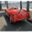
\includegraphics{graphics/automobile6.png}
        \caption{Automobile}
        \label{subfig:automobile6}
    \end{subfigure}
    \begin{subfigure}{.32\linewidth}
        \centering
        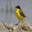
\includegraphics{graphics/bird9.png}
        \caption{Bird}
        \label{subfig:bird9}
    \end{subfigure}
    \caption{Example CIFAR-10 Images}
    \label{fig:examples}
\end{figure}

\subsection{Benign \& Malicious Models}\label{subsec:benignmalicious}

For the target classification models, we use a 34-layer Residual Network (ResNet) based largely on previous work from Kaiming He et al \cite{DBLP:journals/corr/HeZRS15}.  A visualization of the ResNet structure is shown in Appendix \ref{app-ResNet}.  The training step consists of 200 epochs using a batch size of 16 images/labels.  For the malicious models, the training data is augmented with a malicious data set as follows:

\begin{enumerate}
    \item $N_T$ target images are selected from the benign training set for later ex-filtration, and encoded as a vector of image labels $Y_mal$.  We chose $N_T = 1$ for this paper.  The size (number of labels) of the resulting label vector is: 
    \begin{align*}
        \lvert Y_{mal} \rvert = & \frac{N_T \times size_{image} \times n_{channels} \times 8}{\lfloor log_2(n_{categories}) \rfloor} \\
        = & \frac{1 \times 32 \times 32 \times 3 \times 8}{\lfloor log_2 10 \rfloor} = 8,192
    \end{align*}
    \item A pseudo-random number generator is seeded with a known (to the malicious ML provider) value.  We choose $47405$, the zip code for IU Bloomington.
    \item $X_{mal}$ is generated as a set of $\lvert Y_{mal} \rvert$ pseudo-random images of size $32 \times 32 \times 3$.
    \item The original training set is augmented with $X_{mal}$ and $Y_{mal}$ data, and trained using the same parameters as the benign model.
\end{enumerate}

In this implementation, since the number of categories isn't a power of two, then there are some categories (categories 8 and 9) that are never used as labels by the malicious encoder.  This is a potential red herring for a malicious model classifier, but is easily circumvented by the malicious ML provider by either choosing by an encoding number base that is equal to the number of categories (if the provider knows the number of categories a priori) or perhaps adding a pseudo-random number to the malicious labels (then modulo the number of categories) so that each category gets equivalent representation.

Table \ref{tab:good-bad-model-performance} shows the performance that was achieved on both $M_{T_{ben}}$ and $M_{T_{mal}}$ for the benign classification task.  The performance for $M_{T_{mal}}$ is worse because the real training set containing 25,000 images is diluted with with 8,192 malicious images trained to meaningless labels, from the benign classification task's perspective.  In other words, the malicious data augmentation serves to add considerable noise to the data.  Additional effort could be applied to better generalize the model, but for the purposes of this paper, ~70\% accuracy is acceptable performance.

\begin{table}[ht]
    \caption{Classification Model Performance}
    \label{tab:good-bad-model-performance}
    \begin{tabular}{l|c|c}
        \toprule
        Model       &Trng. Accuracy    &Val. Accuracy \\
        \midrule
        Benign      &0.9924            &0.7276 \\
        Malicious   &0.9918            &0.6992\footnote{The malicious model was validated against authentic CIFAR-10 validation data, not malicious data.} \\
        \bottomrule
    \end{tabular}
\end{table}

To extract the secret image from $M_{T_{mal}}$, we need only possess the seed value for the pseudo-random number generator in order to reproduce the malicious training images $X_{mal}$.  The images are produced and presented to $M_{T_{mal}}$ for classification.  The highest-probability labels are taken from the resulting prediction vectors and then decoded to a $32 \times 32 \times 3$ image by essentially reversing the encoding scheme described above.  Some original and corresponding ex-filtrated (using a malicious model) images are shown in Figure \ref{fig:exfil-images}.  For comparison, an original and its corresponding ex-filtrated image using a benign model is shown in Figure \ref{fig:un-exfil-images}.

\begin{figure}
    \begin{subfigure}{.49\linewidth}
        \centering
        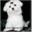
\includegraphics[scale=2]{graphics/M00_hdf5_original.png}
        \caption{Original}
        \label{subfig:M00-orig}
    \end{subfigure}
    \begin{subfigure}{.49\linewidth}
        \centering
        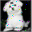
\includegraphics[scale=2]{graphics/M00_hdf5_exfil.png}
        \caption{Exfil}
        \label{subfig:M00-exfil}
    \end{subfigure}
    \begin{subfigure}{.49\linewidth}
        \centering
        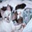
\includegraphics[scale=2]{graphics/M01_hdf5_original.png}
        \caption{Original}
        \label{subfig:M01-orig}
    \end{subfigure}
    \begin{subfigure}{.49\linewidth}
        \centering
        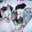
\includegraphics[scale=2]{graphics/M01_hdf5_exfil.png}
        \caption{Exfil}
        \label{subfig:M01-exfil}
    \end{subfigure}
    \caption{Malicious Model Ex-Filtration}
    \label{fig:exfil-images}
\end{figure}

\begin{figure}
    \begin{subfigure}{.49\linewidth}
        \centering
        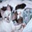
\includegraphics[scale=2]{graphics/G01_hdf5_original.png}
        \caption{Original}
        \label{subfig:G01-orig}
    \end{subfigure}
    \begin{subfigure}{.49\linewidth}
        \centering
        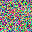
\includegraphics[scale=2]{graphics/G01_hdf5_exfil.png}
        \caption{Exfil}
        \label{fig:G01-exfil}
    \end{subfigure}
    \caption{Benign Model Ex-Filtration }
    \label{fig:un-exfil-images}
\end{figure}

\subsection{Malicious Inference}
At this point in the threat scenario, the client has submitted their data $(X, Y)$, received the resulting model $M_{T}$, and would like to know whether $M_{T}$ is benign or malicious.  Our approach to achieve this result loosely follows the Membership Inference Attack approach described in \cite{DBLP:journals/corr/ShokriSS16} and is graphically depicted in \ref{app-approach}.

\begin{enumerate}
    \sloppy
    \item Select multiple subsets of the CIFAR-10 data set to use for shadow models, referred to as $\{D_0, D_1, ...D_{m-1}\}$ where $D_i: (X_{i_{trn}}, Y_{i_{trn}}), (X_{i_{tst}}, Y_{i_{tst}}) \mid i \in \{0, 1, ..., m-1\}$.  The shadow models generated for this paper used 20\%, randomly selected, of the second half of the CIFAR-10 data set (as loaded using \texttt{keras.datasets.cifar10.load\_data()}), or 5,000 and 1,000 image-label pairs for $(X_{i_{trn}}, Y_{i_{trn}})$ and $(X_{i_{tst}}, Y_{i_{tst}})$, respectively.
    \item Using the methodology from section \ref{subsec:benignmalicious} above and the training portion of each data set $(X_{i_{trn}}, Y_{i_{trn}})$, generate benign / malicious shadow model pairs $(M_{i_{ben}}, M_{i_{mal}})$ corresponding to each data set.  The approach used herein assumes the shadow models are similar in structure to the target model.
    \item Using $m-1$ newly-generated pseudo-random image sets $X_{i_{rnd}} \mid i \in \{0, 1, ..., m-1\}$, obtain a complete set of prediction vectors $P_s$ from all benign and malicious shadow models applied to their corresponding set of random images in $X_{i_{rnd}}$. So, $P_s = M_{0_{ben}}(X_{0_{rnd}}) \cup M_{0_{mal}}(X_{0_{rnd}}) \cup ... \cup M_{{m-1}_{ben}}(X_{{m-1}_{rnd}}) \cup M_{{m-1}_{mal}}(X_{{m-1}_{rnd}})$
    \item The resulting prediction vectors in $P_s$ form the base features $X_a$ upon which a new attack model $M_{a}$ can be developed.  The labels for said features $Y_a$ are assigned to be $0$ if the prediction vector came from a benign model, and $1$ if from a malicious model.  This new data set is split into a training and test subset, described as $D_{a}: \{(X_{a_{trn}},Y_{a_{trn}}), (X_{a_{tst}},Y_{a_{tst}})\}$.
    \item $X_a$ can be pre-processed or augmented with additional features derived from the base features. For this work, prediction values for the last two categories $(p_8, p_9)$ were removed from $X_a$ since they were not used in the encoding process and thus may artificially enhance $M_a$'s ability to predict maliciousness. Additionally, the element-wise variance (var of each prediction vector) was calculated and added as a new feature $var_e$. 
    \item Perform Logistic Regression using the (optionally preprocessed) training set $(X_{a_{trn}},Y_{a_{trn}})$ resulting in the attack model $M_a$.  Per \cite{Simple-LR-Keras}, Keras was used to instantiate the Logistic Regression model.
\end{enumerate}

The structure of the resulting Logistic Regression model $M_a$ is shown in Figure \ref{fig:LR-model} below.

\begin{figure}[H]
    \centering
    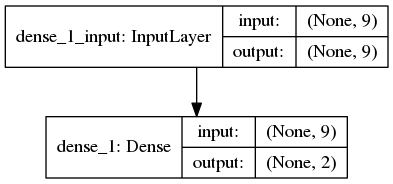
\includegraphics[scale=0.4]{graphics/atkmodel.png}
    \caption{Attack Model Structure}
    \label{fig:LR-model}
\end{figure}

$M_a$ can now be applied to any prediction vector that results from any model responding to any random 32x32x3 image and will predict whether or not that model is benign or malicious.

\section{Results}

During the Logistic Regression step, the attack model $M_a$ achieved 84\% accuracy on both the training set $(X_{a_{trn}},Y_{a_{trn}})$ and the validation set $(X_{a_{tst}},Y_{a_{tst}})$.  Against the original Benign and Malicious models $M_{T_{ben}}$ and $M_{T_{mal}}$, and using a threshold probability of 0.5, the Attack model $M_a$ correctly classified 99\% and 80\% of the responses as having come from $M_{T_{ben}}$ and $M_{T_{mal}}$, respectively.  In other words, against $M_{T_{ben}}$, 99\% of responses to random inputs will be correctly classified as having come from $M_{T_{ben}}$.  Against $M_{T_{mal}}$, 80\% of responses to random inputs will be correctly classified as having come from $M_{T_{mal}}$.  Shown in Figure \ref{fig:results_hist} below is histogram visualizing the $M_a$'s performance.

\begin{figure}[H]
    \centering
    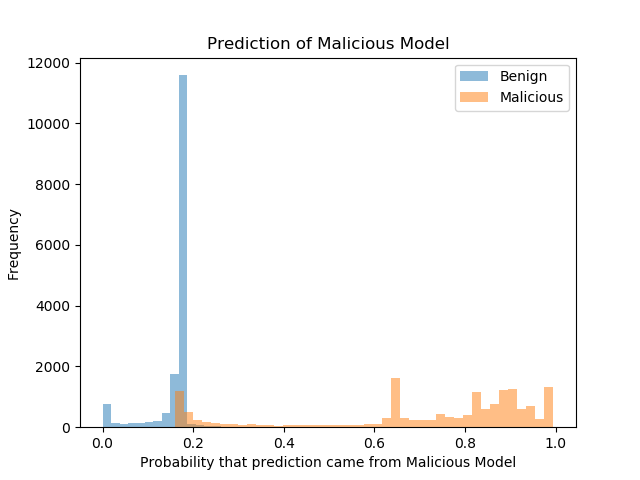
\includegraphics[scale=0.4]{graphics/results_200e.png}
    \caption{Histogram of Attack Model Performance}
    \label{fig:results_hist}
\end{figure}



\section{Conclusions}

An important assumption behind this work is that the ML client has knowledge of the target model's structure or can generate multiple known-good and known-malicious shadow models.  That assumption limits the utility of this work because, obviously, if the ML client can generate known-good models or has knowledge of the model's structure, what need does s/he have of the ML provider?  Nevertheless, this work demonstrates that methods exist today that can detect differences in model behavior outside of the space that is occupied by the relevant data set, to include possible detection of malicious behavior.

\section{Future Work}

This paper captures a minimal research effort to demonstrate that a variation of the Membership Inference Attack can be used to detect whether a given machine learning model may have a covert channel. Future work would be to investigate whether a single Attack model (say a ResNet) might be used to detect covert channels in other target models with different structures, but the same classification task.  Additional efforts might look at whether the process is generalize-able such that simple shadow models can be used to build Attack models that are effective against complex target models, or otherwise characterize `good' and `bad' behavior of any model based only on it's assigned task and achieved performance.  Future research of this nature may extend the core concepts described herein into more realistic threat scenarios, as well as serve to inform future research on the nature and behavior of models, their capacity, and their defined and undefined behavior.


\begin{acks}

The authors acknowledge the Indiana University Pervasive Technology Institute for providing Big Red II resources that have contributed to the research results reported within this paper \cite{PTI}.

This research was supported in part by Lilly Endowment, Inc., through its support for the Indiana University Pervasive Technology Institute, and in part by the Indiana METACyt Initiative. The Indiana METACyt Initiative at IU was also supported in part by Lilly Endowment, Inc.

\end{acks}

\newpage
\appendix
%\newpage
%Appendix A
\section{Structure of 34-Layer Residual Network} \label{app-ResNet}

See Figure \ref{fig:model}.

\begin{figure*}[ht]
    \centering
    \begin{subfigure}{.24\linewidth}
    \centering
        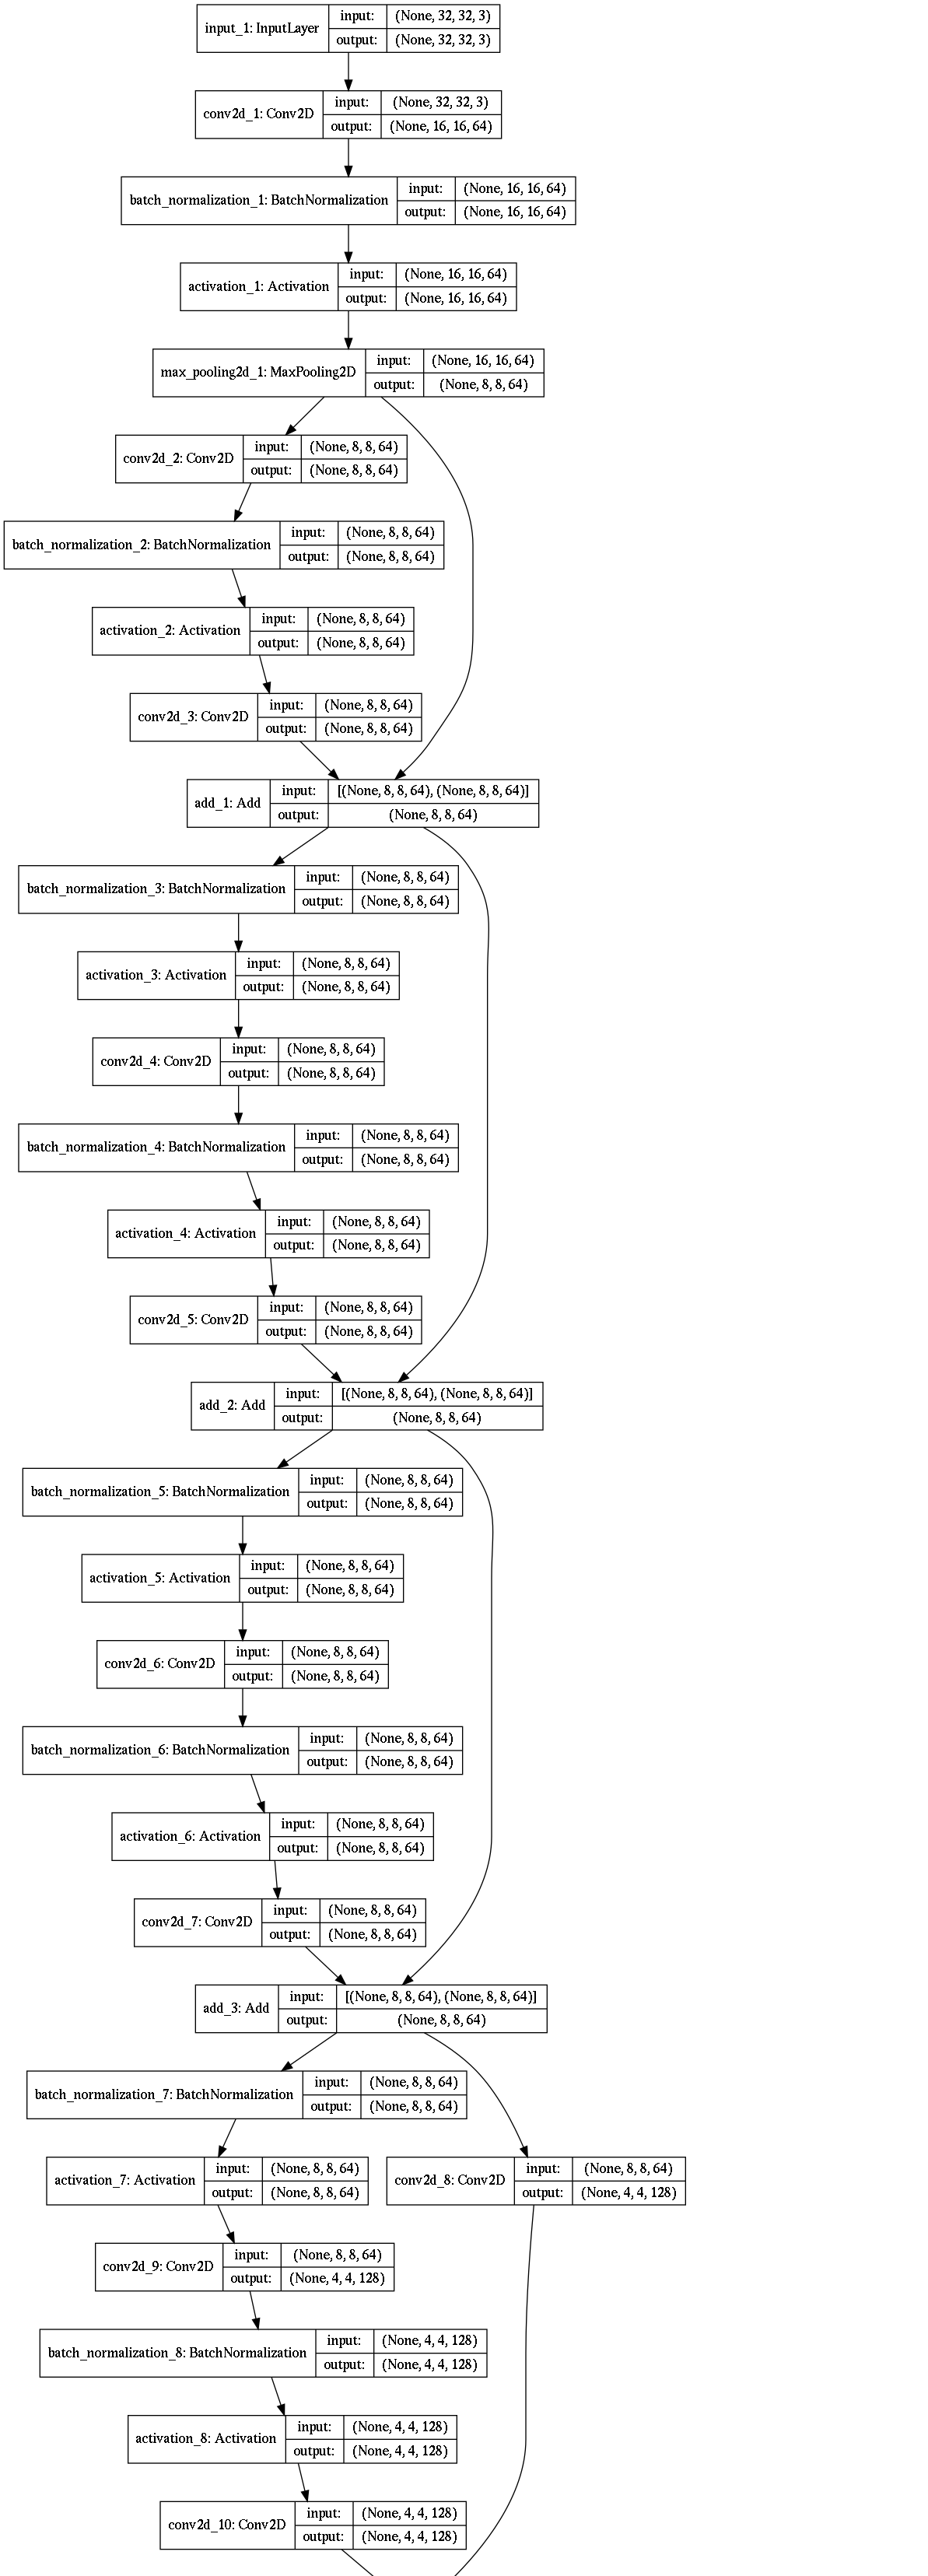
\includegraphics[scale=.1]{graphics/model_cropped_0.png}
        %\caption{Model}
        \label{subfig:model0}
    \end{subfigure}
    \begin{subfigure}{.24\linewidth}
    \centering
        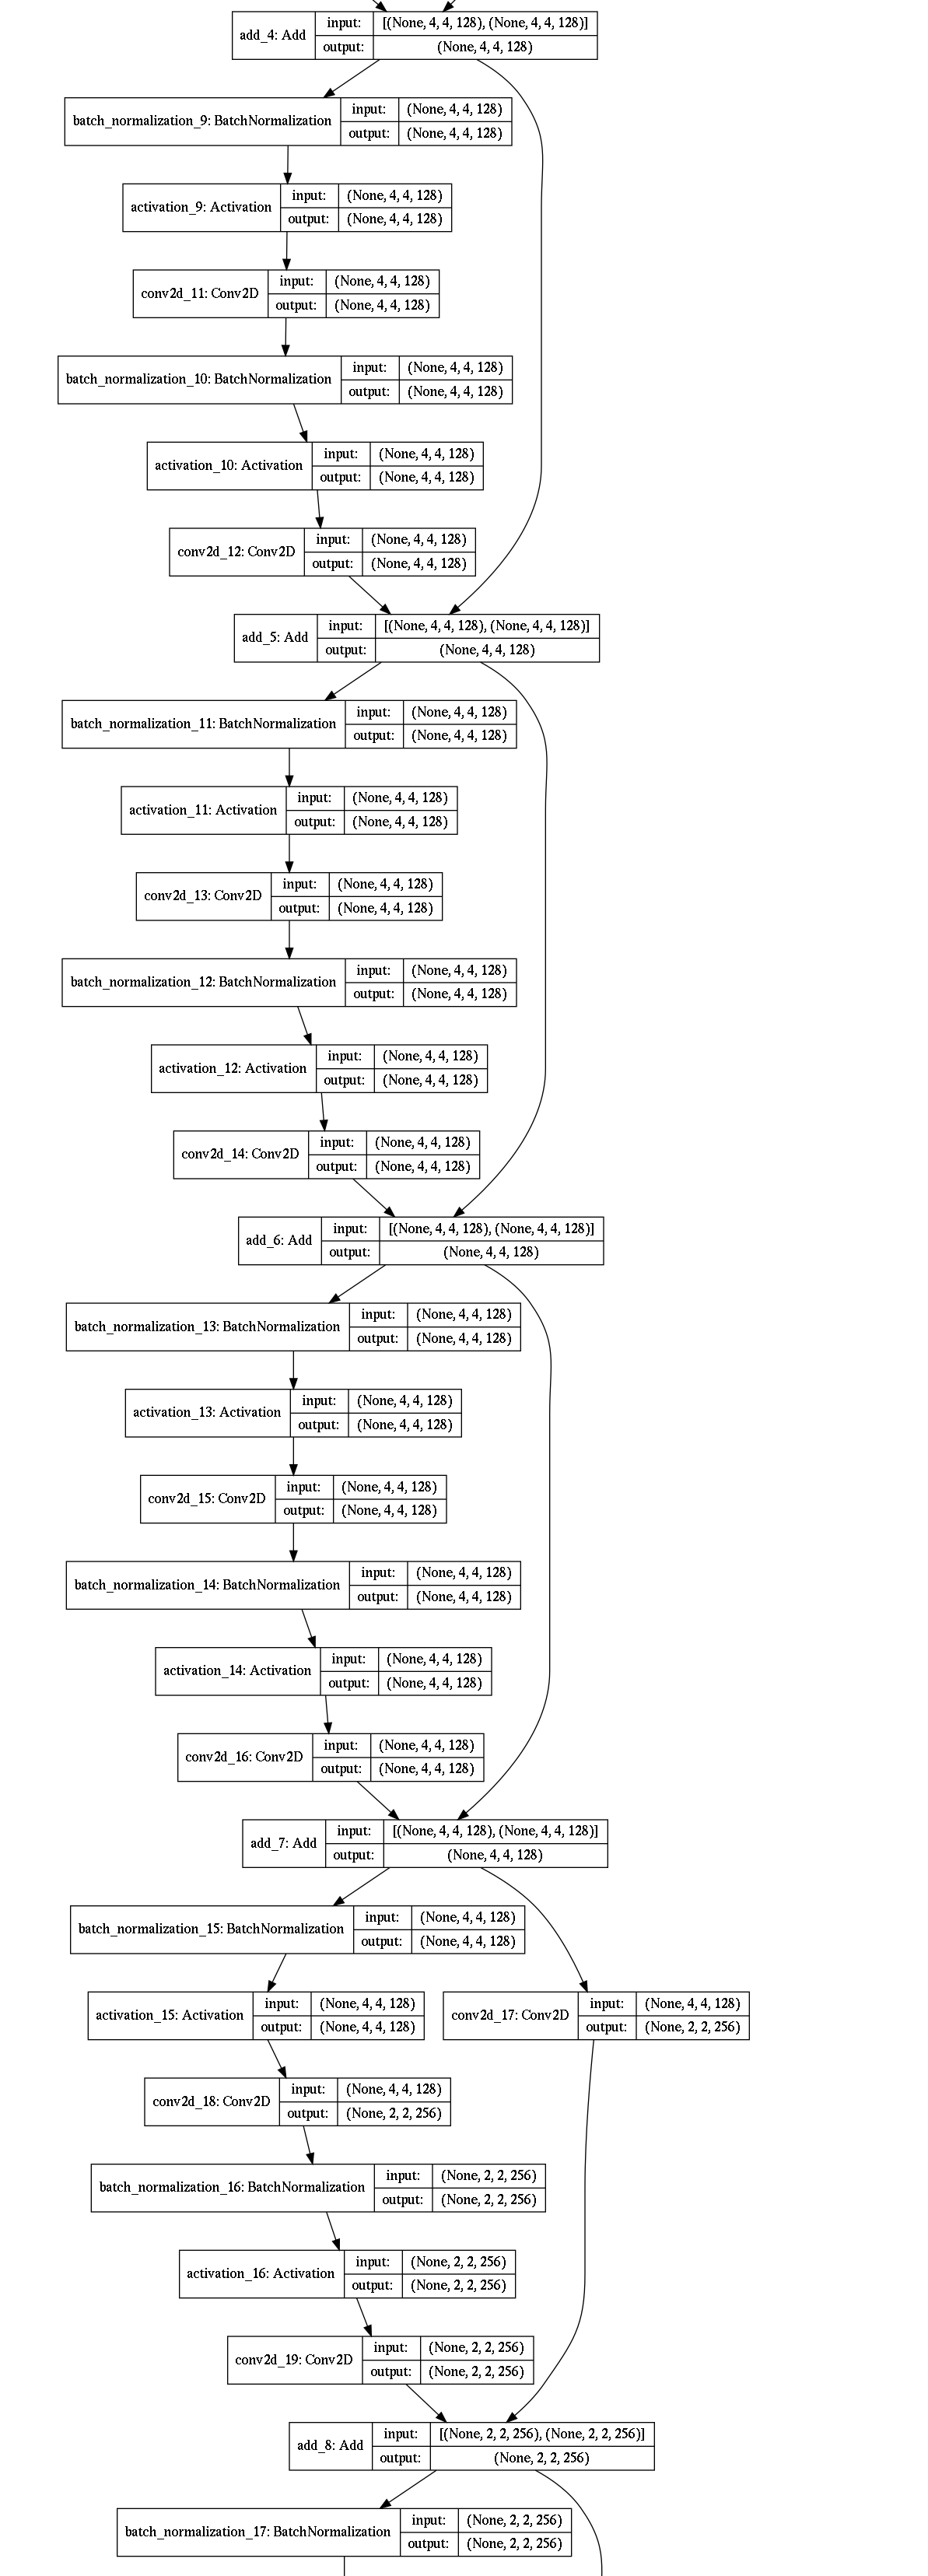
\includegraphics[scale=.1]{graphics/model_cropped_1.png}
        %\caption{Automobile}
        \label{subfig:model1}
    \end{subfigure}
    \begin{subfigure}{.24\linewidth}
    \centering
        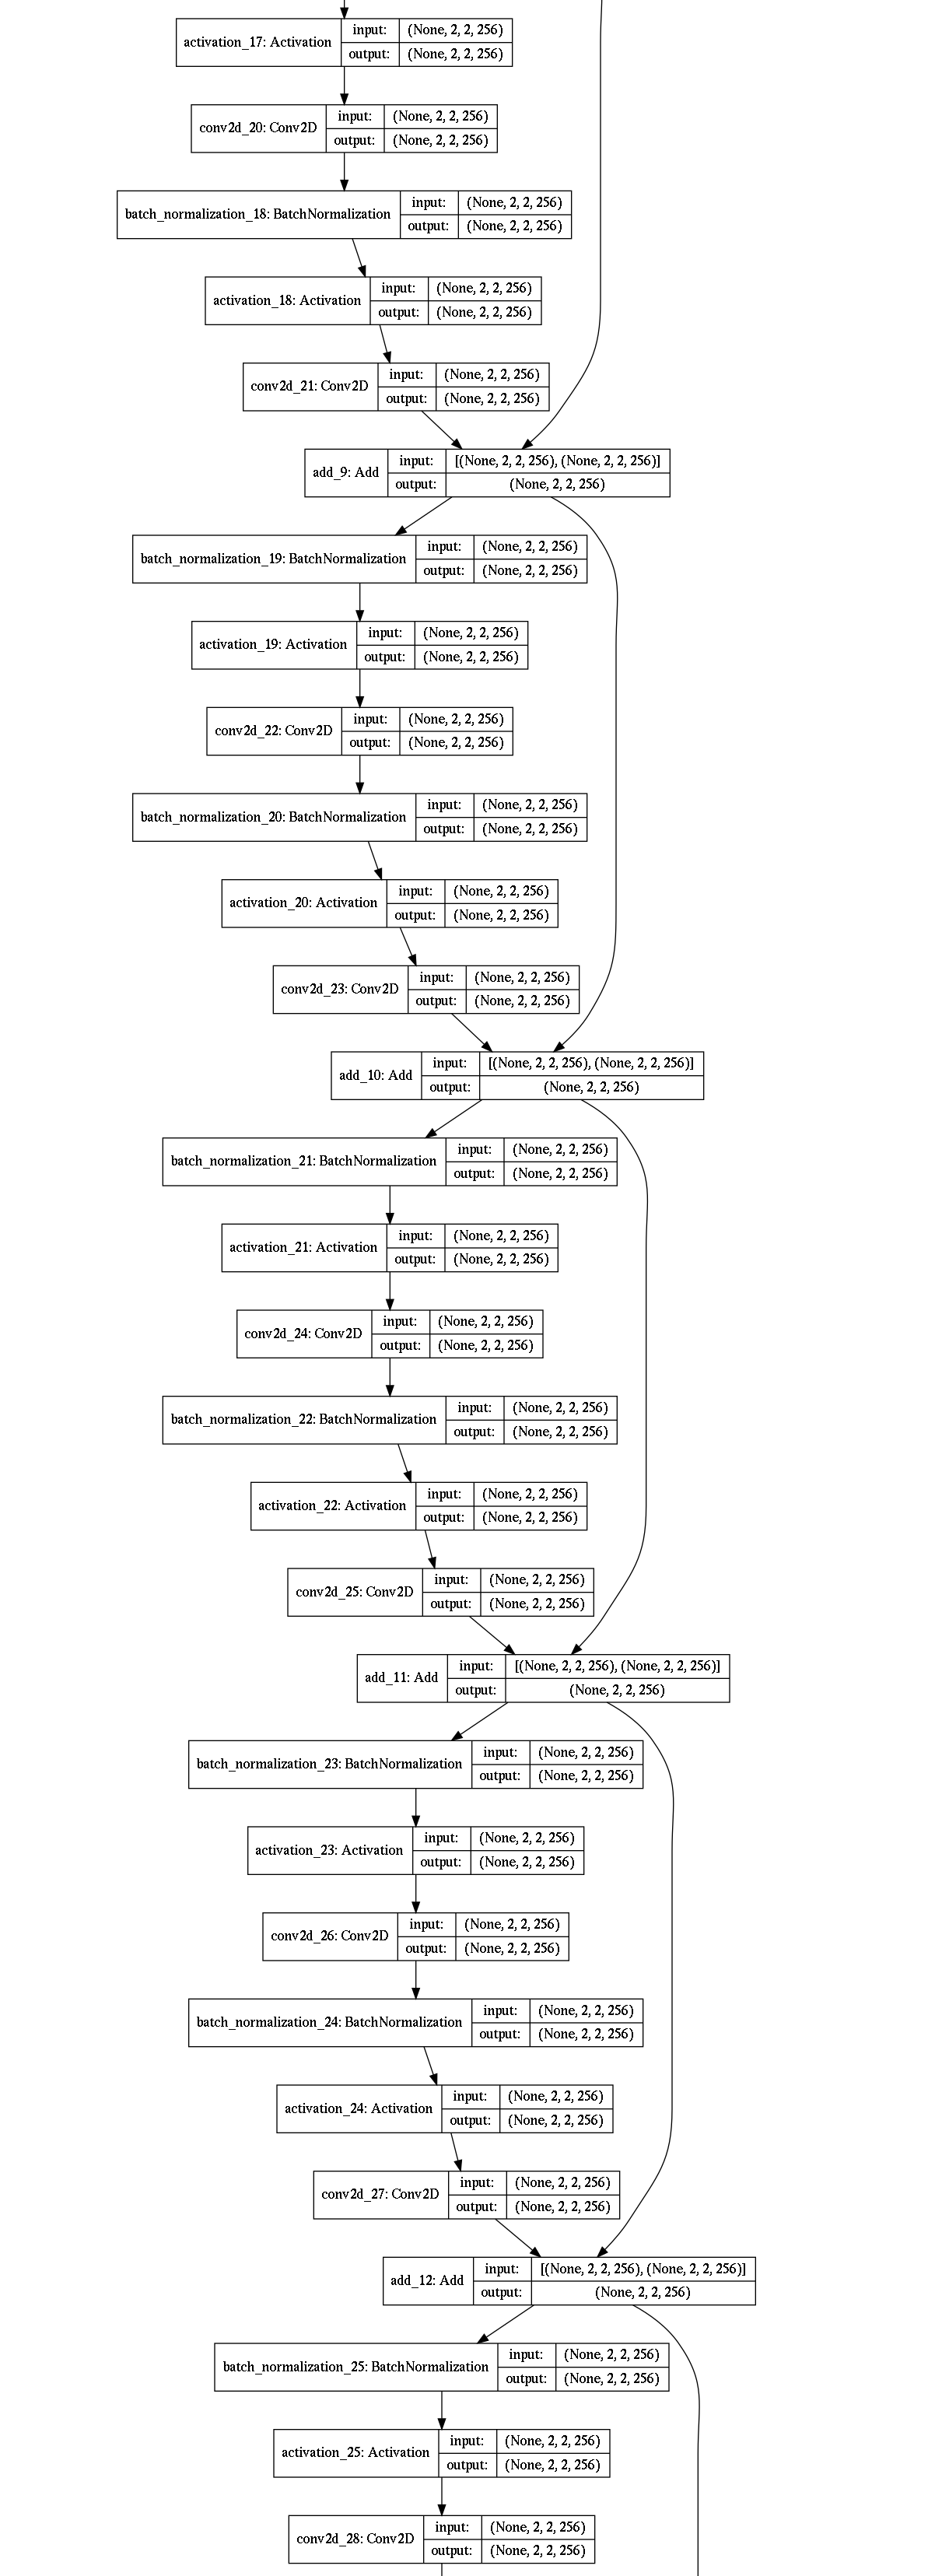
\includegraphics[scale=.1]{graphics/model_cropped_2.png}
        %\caption{Bird}
        \label{subfig:model2}
    \end{subfigure}
    \begin{subfigure}{.24\linewidth}
    \centering
        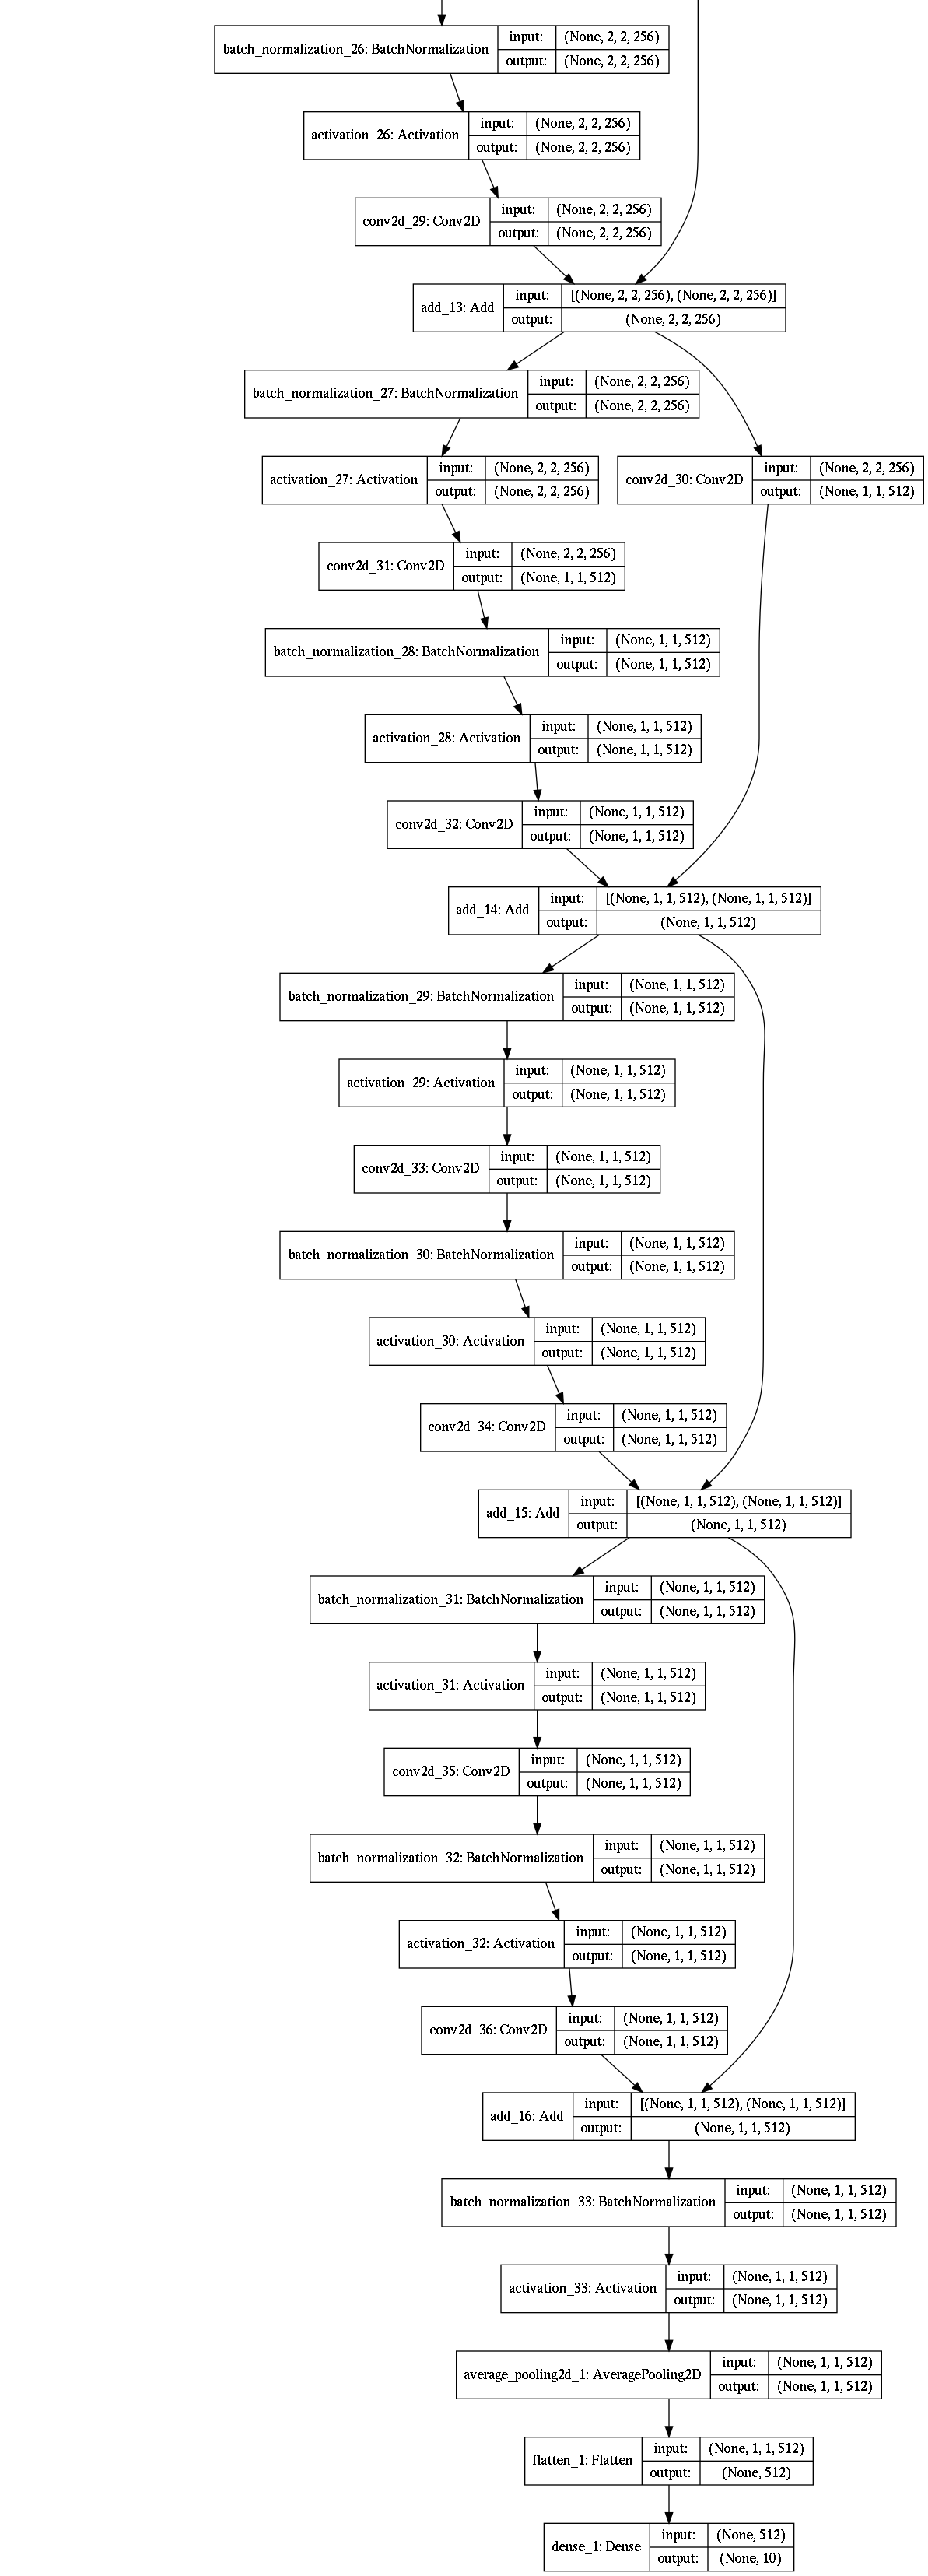
\includegraphics[scale=.1]{graphics/model_cropped_3.png}
        %\caption{Bird}
        \label{subfig:model3}
    \end{subfigure}
    \caption{ResNet Model Structure}
    \label{fig:model}
\end{figure*}


%Appendix B
\section{Overall Approach} \label{app-approach}

See Figure \ref{fig:concept}.

\begin{figure*}[ht]
    \centering
    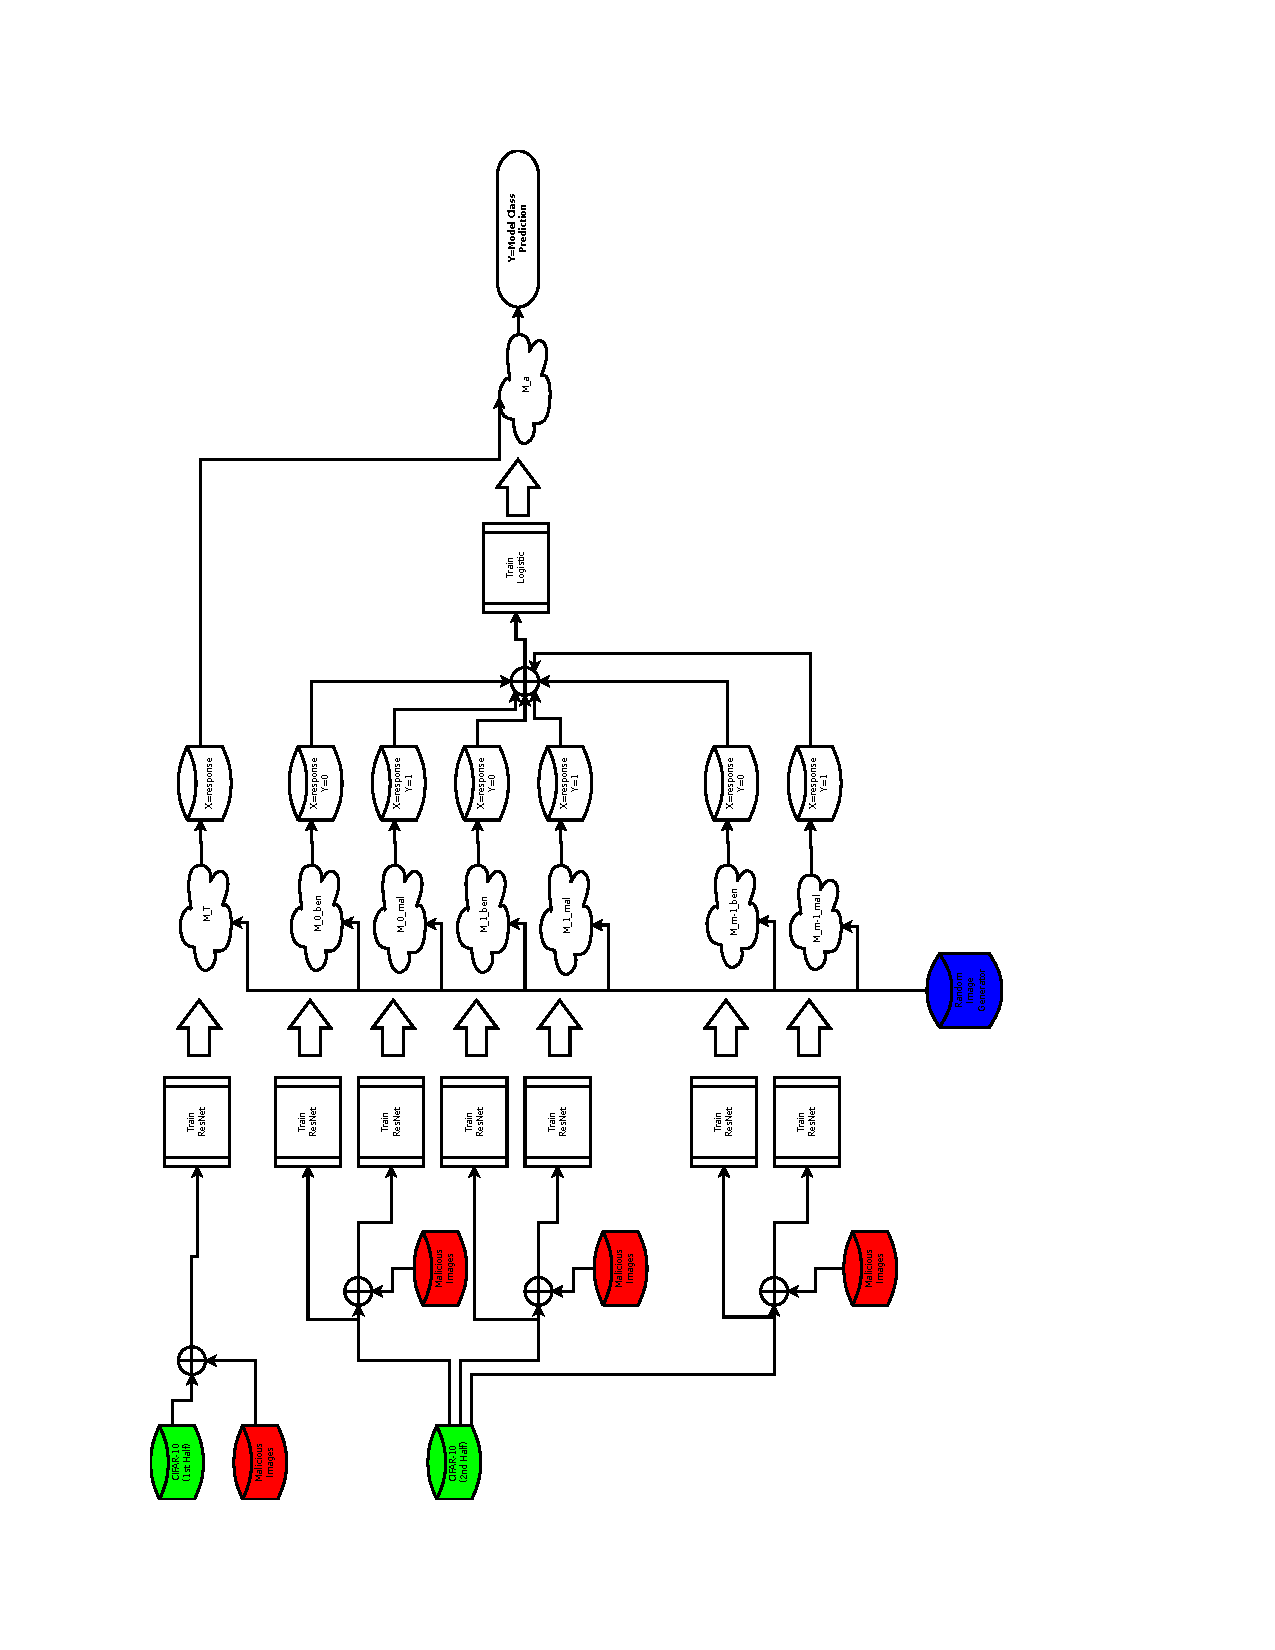
\includegraphics[scale=0.6, angle=-90, trim={2cm 2cm 4cm 2cm}, clip]{graphics/Concept_r1.pdf} %{t l b r}
    \caption{Membership Inference Approach to Covert Channel Detection}
    \label{fig:concept}
\end{figure*}






\bibliographystyle{ACM-Reference-Format}
\bibliography{bibliography}

\end{document}
